\documentclass[a4paper]{article}

\usepackage{graphicx}
\usepackage{subfigure}
\usepackage{caption}
\usepackage[utf8]{inputenc}
\usepackage{amsmath}
\usepackage{amsfonts}
\usepackage{amssymb}
\usepackage{amsthm}
\usepackage[german]{babel}
\title{Zwisschenberichte FOUNTT}
%\author{Stefano Di Lucia}
%\date

\begin{document}
\maketitle

Die Ziele dieses Teilarbeitspakets sind
\begin{itemize}
\item die Schnittstellenspezifikation und Hardwarespezifikation des UAVs; 
\item die Datenaufnahme eines beispielhaften Tr"ummerfeldes nach einer Naturkatastrophe.
\end{itemize}
Das Anwendungsszenario des Systems ist der Katastropheneinsatz, in dem das UAV einen optimalen Landeplatz finden und dort autonom landen soll. Die Aufgabe des UAVs ist es, nach der Landung eingeschlossene und versch"uttete Menschen zu lokalisieren.
   

\section*{Hardwarespezifikationen} 
Um diese Aufgabe zu erf"ullen, ben"otigen wir einen Quadrotor mit verschiedenen Sensoren: 
\begin{itemize}
\item Lagesensoren (z.B. IMU, GPS), um die Drohne stabil in der Luft zu halten. 
\item Stereokamera, die zur Rekonstruktion dreidimensionaler Oberfl"achen und der Landeplatzsuche eingesetzt wird.
\item BioRadar zur Lokalisierung versch"utteter Menschen unter Tr"ummerteilen. 
\end{itemize}
Nach sorgf"altiger Suche w"ahlten wir die DJI MATRICE 100 Drohne. 
Das ist eine vollwertige, frei programmierbare Flugplattform mit der M"oglichkeit, die Laufzeit durch eine zweite Batterie zu verl"angern.
\begin{center}
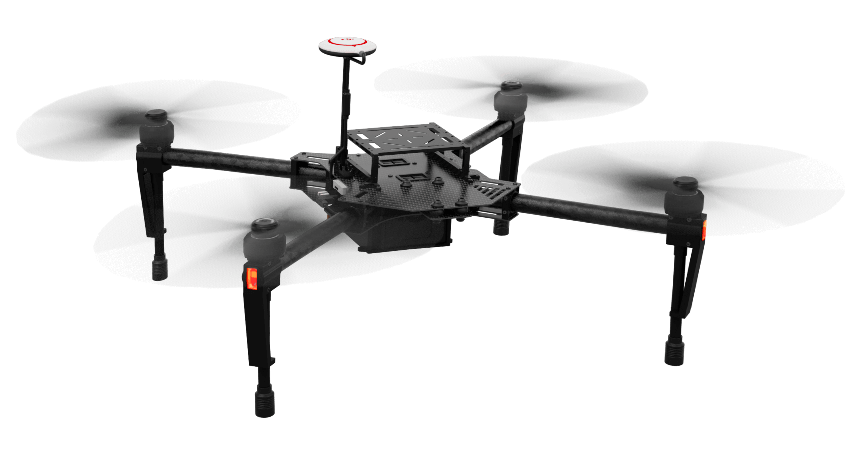
\includegraphics[width=0.8\textwidth]{Matrice_100.png}
\end{center}
Das von uns gew"ahlte System enth"alt neben der Flugsteuerung auch GPS- und IMU-Sensoren, die zur Erf"ullung der oben aufgef"uhrten Anforderungen ben"otigt werden.

\begin{center}
\begin{tabular}{ c | c }
\hline
\multicolumn{2}{c}{Technische Spezifikationen DJI MATRICE 100}\\
\hline
Diagonal Wheelbase & $650mm$\\
Gewicht (mit Batterie) & $2431g$\\
Max. Takeoff Gewicht & $3600g$\\
Hovering Time & No payload: $28 min$, $1Kg$ payload: $16 min$
\end{tabular}
\end{center}

Mit der ZED 2k Stereo Camera w"ahlten wir einen Sensor, der sowohl f"ur Depth Sensing (Tiefenmessung) als auch Motion Tracking (Bewegungsverfolgung) geeignet ist. 
\begin{center}
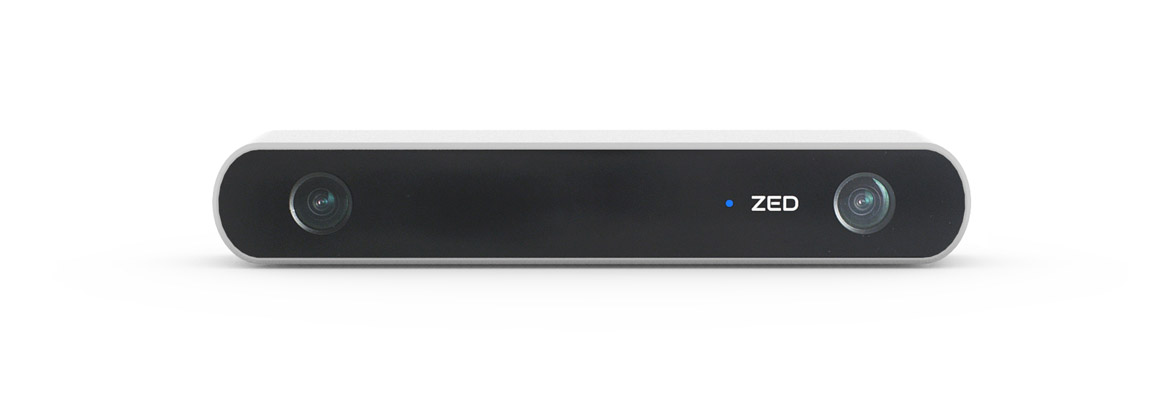
\includegraphics[width=0.8\textwidth]{ZED_camera.jpg}
\end{center}
Die Kamera hat eine Reichweite von $20m$ und kann f"ur Real-time (Echtzeit-) SLAM im Innen- und Außenbereich eingesetzt werden. 
\begin{center}
\begin{tabular}{ c c }
\hline
\multicolumn{2}{c}{Technische Spezifikationen ZED Kamera}\\
\hline
Dimensionen & $175\times30\times33 mm$\\
Gewicht & $159 g$\\
Stromverbrauch & $5V / 380mA$
\end{tabular}
\end{center}

\begin{center}
\begin{tabular}{ c c c }
\hline
\multicolumn{3}{c}{Video-Einstellungen}\\
\hline
Einstellung & FPS & Aufl"osung\\
$2.2K$ & $15$ & $4416\times1242$\\
$1080p$ & $30$ & $3840\times1080$\\
$720p$ & $60$ & $2560\times720$
\end{tabular}
\end{center}

In Erg"anzung halten wir das Jetson TX1 Embedded Systems Modul f"ur sinnvoll.
\begin{center}
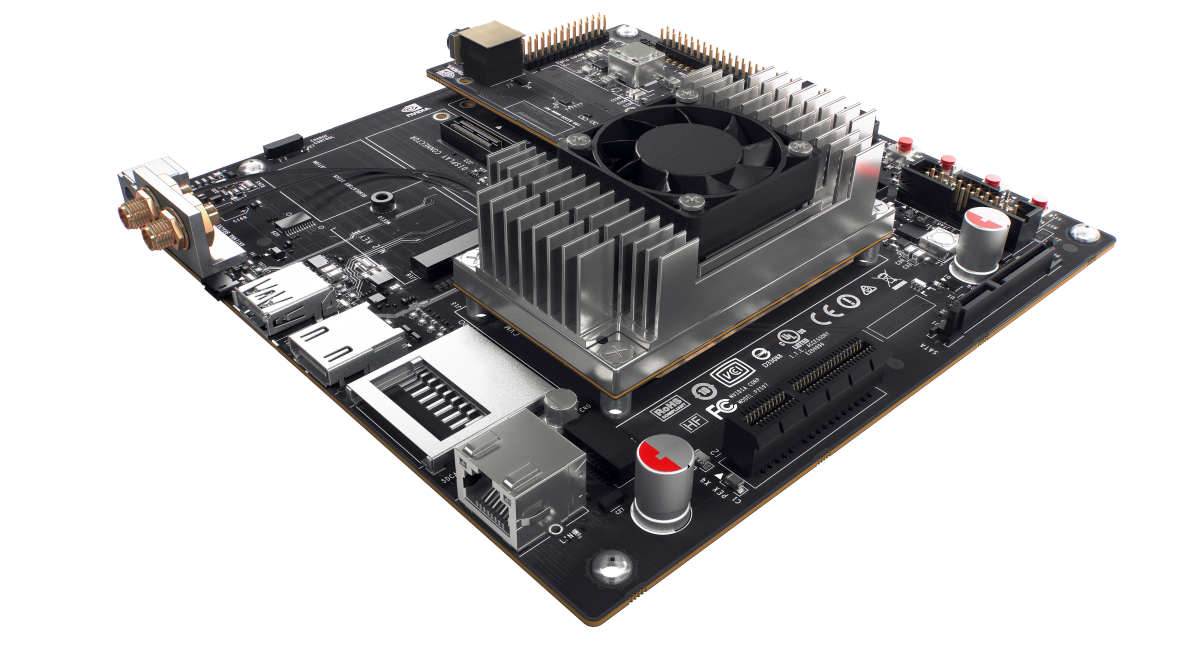
\includegraphics[width=0.8\textwidth]{JetsonTX1.png}
\end{center}
Das TX1 ist eine Entwicklungsplattform f"ur Deep-Learning- und Computer-Vision-Anwendungen sowie Berechnungen auf der Grafikkarte. Mit diesem System k"onnen Stereo-Kameradaten verarbeitet und on-line Neuronale Netze f"ur die autonome Landung ausgewertet werden.
\begin{center}
\begin{tabular}{ c | c }
\hline
\multicolumn{2}{c}{Technische Spezifikationen Jetson TX1}\\
\hline
GPU & NVIDIA Maxwell\textsuperscript{TM} 256 CUDA Cores\\
CPU & Quad-core ARM Cortex-A57 MPCore Prozessor\\
Speicher & 4 GB LPDDR4 \\
Stromverbrauch & Leerlauf: $1-2W$, unter Arbeitsbelastung: $6-10W$\\
Gewicht & $350g$
\end{tabular}
\end{center}
Das gesamte, auf die Drohne zu montierende System wird durch die Kamera, das Jetson TX1 und die TX1-Batterie gebildet. Das Gesamtgewicht ist $720g$. Damit ist eine Akkulaufzeit im Schwebezustand von etwa $20 min$ zu erwarten. Es gibt die Moglichkeit mit einer zweiten Batterie die Laufzeit von etwa $30 min$ zu erh"ohen.
%\newpage
\section*{Datenaufnahme} 
Es ist geplant, die oben genannten System in n"achsten Monat zu kaufen und zusammenbauen. Als "Ubergangsl"osung in der Abwesenheit eines passenden Szenarios, montierten wir eine Kamera auf die Parrot 2.0 Drohne und verwendeten ein kleines, k"unstliches Tr"ummerfeld in unserem Labor.
\begin{figure}[h]
\centering
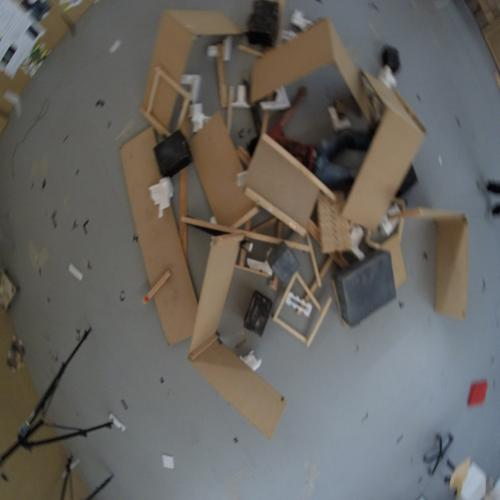
\includegraphics[width=0.4\textwidth]{G0020587.JPG} %
\qquad\qquad
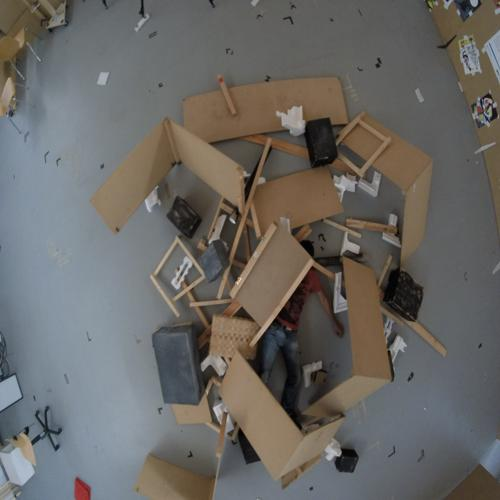
\includegraphics[width=0.4\textwidth]{G0020592.JPG}\vspace{3mm}
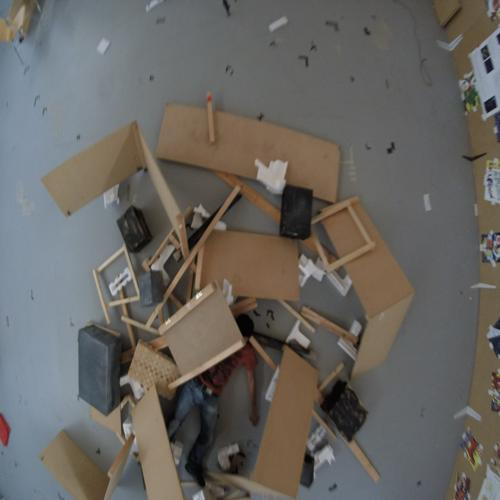
\includegraphics[width=0.4\textwidth]{G0020628.JPG} %
\qquad\qquad
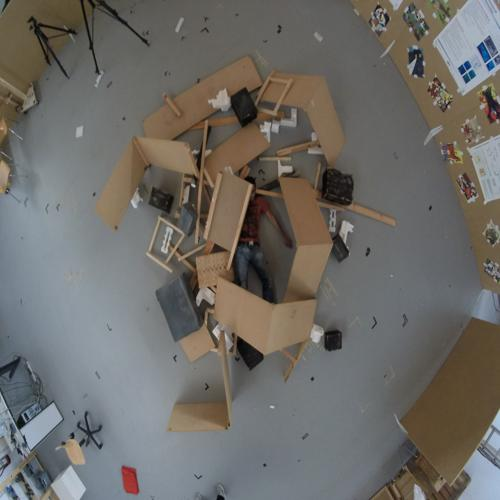
\includegraphics[width=0.4\textwidth]{G0020651.JPG}
\end{figure}
%\begin{figure}[h]
%\centering
%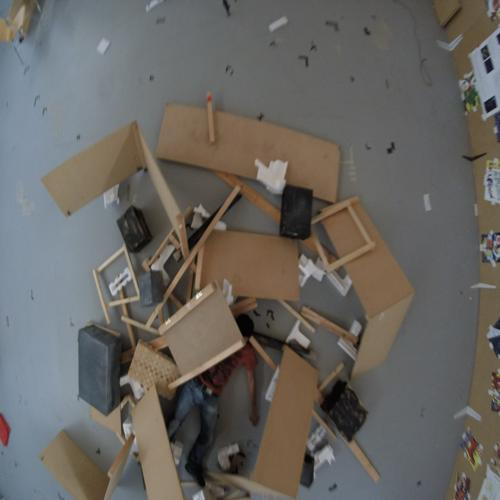
\includegraphics[width=0.42\textwidth]{G0020628.JPG} %
%\qquad\qquad
%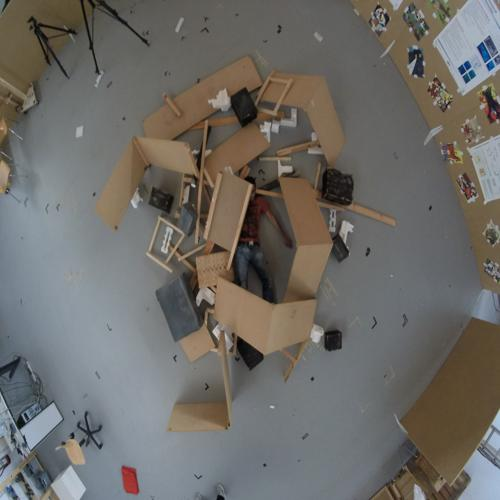
\includegraphics[width=0.42\textwidth]{G0020651.JPG}
%\end{figure}

Wir wollen verschidene Szenario in unserem Labor nachbilden, damit unseres System und Landung Methode ohne Risiko f"ur dritte zu testen. Auf diese Weise ist es m"oglich, Experimente unter Umgebungs- und Beleuchtungsbedingungen zu durchf"uhren. 

Im n"achsten Schritt wollen wir die Daten eines realitischen Einsatzszenarios zu sammeln.
F"ur den kommenden M"arz/April ist geplant, das System in Amatrice zu mitbringen, wo am 26. Oktober 2016 ein Erdbeben war.
\vspace{5mm}
\begin{figure}[h]
%\centering
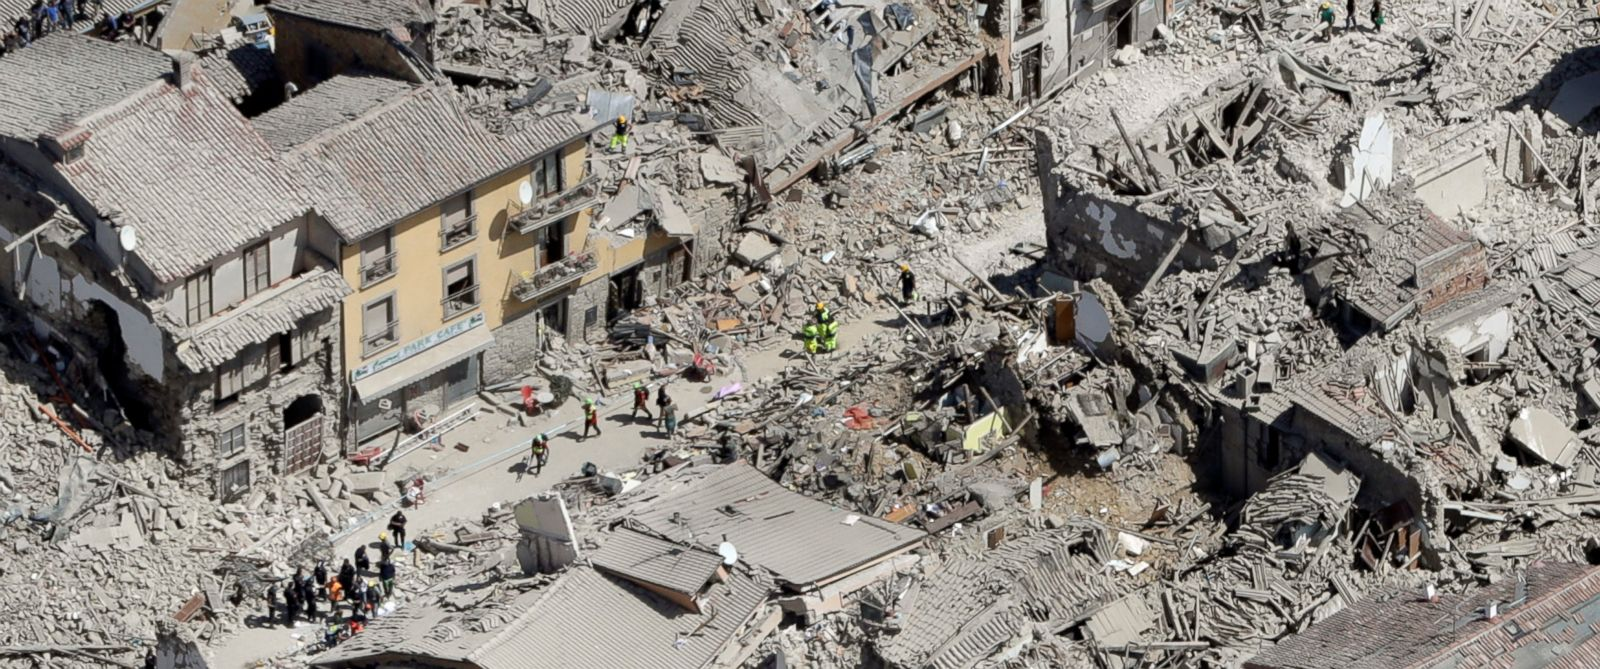
\includegraphics[width=1\textwidth]{Amatrice.jpg}
\captionsetup{labelformat=empty}
\caption{Amatrice nach dem Erdbeben 26. Oktober 2016}
\end{figure}
 
Das Gebiet des Erdbebens ist ziemlich groß und wir k"onnen eine große Anzahl von Trai-
ningsdaten sammeln und untersuchen. Die Manuelle Annotation und Erweiterung vieler Bildern von verschidene zusammengebrochene Gebäude ist wesentlich, ein neuronales Netz für die Erkennung von Landeplätzen zu trainieren. 
Weiterhin ist es m"oglich, in einem verschidenen Dorf in der N"ahe von Amatrice (wie z.B. Arquata del Tronto oder Accumuli) die zuverlässigkeit der Training zu testen .


\end{document}